\documentclass[11pt,a4paper]{article}
\usepackage{listings}
\usepackage{xcolor}
\usepackage{graphicx}

\lstset{
numbers=left,
framexleftmargin=12mm,
frame=none,
backgroundcolor=\color[RGB]{245,245,245},
keywordstyle=\bf\color{blue},
identifierstyle=\bf,
numberstyle=\color[RGB]{0,192,225},
commentstyle=\it\color[RGB]{0,96,96},
stringstyle=\rmfamily\slshape\color[RGB]{128,0,0},
showstringspaces=false
stepnumber=1
numbersep=1
}

\begin{document}
\title{Project 5 : Training a Smartcab}
\author{Wenjie Zhang}
\maketitle

\begin{flushleft}
\section{Realize Basic Function}
\end{flushleft}
Make the cab move in the environment, regardless of any problems about optimization in driving. Notice that your cab will provide the following information:

\begin{itemize}
\item Position of the next cross (according to the current position and forward direction)
\item The state of the cross (red or green light, car existing or not)
\item Current deadline (how much time left)
\end{itemize}

\noindent
To complete this task, randomly choose one of the following movement for your cab. (None, forward, left, right) Regardless of the above information, set the deadline in the virtual environment, that is to set enforce\_deadline as False, and watch the behavior of the intelligent cab.

\vspace{3mm}
\noindent
\textbf{Question 1:}  Watch and record the behavior of the intelligent cab when taking random actions. Does it finally achieve the destination? Are there interesting phenomena worth recording?

\vspace{3mm}
\noindent
\textbf{Answer 1:} When I set action as random choice from None, “forward”, “left” and “right”, the cab will do as the choice, however, it takes long to reach the goal, because it just doesn’t have order and waste lots of time looping around a same place. Also, I can see the reward is changing on the up left of the screen with its report of its deadline, inputs, action and reward in the command lines. Following is where I changed the code to make tests.

\begin{lstlisting}[language={Python}]
action=randon.choice([None,"forward","left","right"])
\end{lstlisting}

\begin{flushleft}
\section{Train the Intelligent Cab}
\end{flushleft}
Now that your cab can move in the environment, your next task is to choose a suitable state to build models for the cab and its environment. State variables mainly come from the inputs of current road, but you do not need to show them all. You can explicitly define the states or input some implicit assembles. At every time node, you need to process input, using self.state to update its current state. Still, you should set enforce\_deadline as False to observe how the cab report its state change.

\vspace{3mm}
\noindent
\textbf{Question2:} Which states do you think is suitable to build the model for cab and environment? Why do you think so?

\vspace{3mm}
\noindent
\textbf{Answer2:} I think five states are important to evaluate the cab and environment: (1) the cab’s location, (2) destination, (3)the cab’s heading direction, (4, 5 and 6) the cab’s actions for forward, left and right is safe or not. However, in order to reduce the number of states to train faster, I would more like to combine (1), (2) and (3) as the next\_waypoint, which can very well represent the relationship between the three states and action choice. But according to different traffic rules, whether turning left, turning right and going forward is safe or not are not absolute. So it is better to let the cab itself learn the rules by what it senses. Thus, finally, I could choose the following states: (1) next\_waypoint, (2) light’s condition(red, green) (3,4,5) oncoming, left, and right car’s motion. If the cab’s action makes it closer to the destination without accident, I think it will be positively rewarded, otherwise, if it does nothing or goes farther from the destiny it will be punished a little, but if it breaks the traffic rules or causes accident, it should be severely punished. Since cab’s heading influences the choice of action, though it doesn’t influence rewards directly, it should be considered. This reward mechanism is reasonable it real world and only considers these three states. Following is where I changed the code and the effect.

\begin{lstlisting}[language={Python}]
inputs = self.env.sense(self)
self.next_waypoint = self.planner.next_waypoint()
light=inputs['light']
oncoming=inputs['oncoming']
left=inputs['left']
right=inputs['right']
 
pro_inputs={'Next_waypoint':self.next_waypoint,\
'Light':light,'Oncoming':oncoming, \
'Right':right, 'Left':left}
state=(self.next_waypoint, light, \
oncoming, left, right)
\end{lstlisting}

\begin{figure}[htbp]
  \centering
  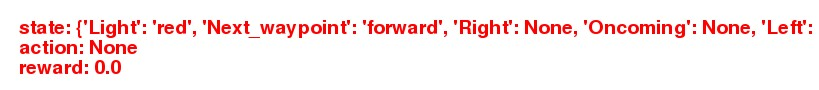
\includegraphics[width=0.9\textwidth]{effect.jpg}
  \caption{Effect after change code}\label{fig:digit}
\end{figure}

\vspace{3mm}
\noindent \textbf{Optional Question:} In this environment, how many states can the cab have? Is the number large enough for us to do Q-Learning for the cab? Tell the reason.

\vspace{3mm}
\noindent \textbf{Answer:} There are 4*4*4*4*2=512 states in this environment, where the first 4 for 4 next way\_points and the following three 4s for conditions of cars from forward, right and left, and 2 for 2 states of light. I think it is large enough for us to do Q-Learning for the cab, since all the conditions are considered for the cab in those states.

\section{Realize Q-Learning Intelligent Cab}
When your intelligent cab is able to understand the input information, and has a map to state, your next task is to realize Q-Learning algorithm for your cab, to make it choose the best action according to current state and the Q values for the action. Every action of the cab will result in a reward based on the environment. Q-Learning cab should update the Q values in when need, considering those rewards. When finishing, set the environment variable enforce\_deadline as True. Run the simulator and observe how the cab moves in every iteration. 

\vspace{3mm}
\noindent \textbf{Question3:}  Compared with randomly choosing actions, what kind of changes do you find in your cab’s actions? Why would those changes happen?

\vspace{3mm}
\noindent \textbf{Answer3:} I think it definitely improved the rate of success, and the cab is smart to obey the traffic rules and go much directly, as I tested. And following is my test method.


\subsection {Set n\_trials=100 before running}
\begin{lstlisting}[language={Python}]
sim.run(n_trials)=100
\end{lstlisting}
\subsection {Define a success\_time in the environment}
\begin{lstlisting}[language={Python}]
valid_actions = [None, 'forward', 'left', 'right']
valid_inputs = {'light': TrafficLight.valid_states, \
'oncoming': valid_actions, 'left': valid_actions, \
'right': valid_actions}
valid_headings = [(1, 0), (0, -1), (-1, 0), (0, 1)]
hard_time_limit = -100
is False, end trial when deadline reaches this value \
(to avoid deadlocks)
success_time=0

print "Environment.act(): Primary agent \
has reached destination!"
self.success_time+=1
\end{lstlisting}
\subsection {Test random actions and result}
\begin{lstlisting}[language={Python}]
action=random.choice(["forward","left","right",None])
\end{lstlisting}
And I got 22 success\_time in 100 tries.
\subsection {Applying Q-learning algorithm agent}
\subsubsection{Initialize state}
\begin{lstlisting}[language={Python}]
deadline = self.env.get_deadline(self)
inputs = self.env.sense(self)
self.next_waypoint = self.planner.next_waypoint()
light=inputs['light']
oncoming=inputs['oncoming']
left=inputs['left']
right=inputs['right']
pro_inputs={'Next_waypoint':self.next_waypoint,\
'Light': light,'Oncoming':oncoming, \
'Right':right, 'Left':left}
state=(self.next_waypoint,light,oncoming,left,right)
self.state=pro_inputs
current_state=state
\end{lstlisting}
\subsubsection{Get next state and reward}
\begin{lstlisting}[language={Python}]
reward = self.env.act(self, action)
#Get next state
inputs = self.env.sense(self)
self.next_waypoint=self.planner.next_waypoint()
light=inputs['light']
oncoming=inputs['oncoming']
left=inputs['left']
right=inputs['right']
pro_inputs={'Next_waypoint':self.next_waypoint,\
'Light': light,'Oncoming':oncoming, \
'Right':right, 'Left':left}
self.state=pro_inputs
state=(self.next_waypoint,light,oncoming,left,right)
next_state=state
\end{lstlisting}
\subsubsection{Update Q values}
\begin{lstlisting}[language={Python}]
self.Qlist.loc[state_dict[current_state],action]=\
(1-self.alpha)*self.Qlist.loc\
[state_dict[current_state],action]+self.alpha*\
(reward+self.gamma*\
self.Qlist.loc[state_dict[next_state]].max())
\end{lstlisting}
\subsubsection{Choose best action}
\begin{lstlisting}[language={Python}]
best_Q=self.Qlist.loc[state_dict[current_state]].max()
action_l=[]
for item in ["forward","left","right",None]:
    if self.Qlist.loc[state_dict[current_state],item]\
    ==best_Q:
        action_l.append(item)
action = random.choice(action_l)
\end{lstlisting}
\subsubsection{Result}

I got 99 success\_time in 100 tries, where alpha=0.5, gamma=0.5, epsilon=0.

\vspace{3mm}
\noindent The test above obviously confirmed my statement that choosing actions according to trained Q values is much better than randomly choosing actions. The reason is that I updated the Q values in the training process, which makes it much more reliable since it was based on experience. Moreover, the immediate reward and long term reward are both considered.

\section{Improve the Q-Learning Intelligent Cab}
In this project, your final task is to improve your intelligent cab, making sure that after enough training, it will achieve the destination in time and safely. Adjust alpha, gamma and epsilon to improve the success rate of your cab.

\vspace{3mm}
\noindent \textbf{Question4:}  Record the processing of adjusting perimeters, which is better? How good is it?

\vspace{3mm}
\noindent \textbf{Answer4:} There are 3 perimeters that I can adjust, learning alpha, gamma and epsilon. 

\noindent Alpha represents for learning rate, which means how fast it will learn. It could not be too small, for example if it is 0, then Q values do not change at all, but it could not be too large, either since if it’s near too 1, then the old Q values are all disregarded, which means it is only one-step learning. So in most cases, I would choose alpha between 0.3-0.7.

\noindent Gamma is the discount value, which controls the future weight to the policy, if it is too small the algorithm would only consider the current reward, which would disregard the long term benefits. But if it is too large, the current benefit is ignored. So I would choose gamma between 0.3-0.7 in most cases, like alpha.

\noindent Epsilon is the exploration rate, which means the rate of randomly choosing action on purpose, since making mistakes would be helpful to learn more. But since the total number of actions is fixed (such as 100 in this case), epsilon should not be too large, either, since besides learning, we also have to apply the policy, or it is meaningless. In a word, the larger the epsilon, the more it learns but the less it uses the policy. As we can still learn when epsilon is small, and randomly choosing would obviously decreasing the current turn’s success possibility, I would choose a small epsilon, in between 0-0.05. Following is my try on different perimeters and the result.

\vspace{3mm}
\noindent I find I can observe the cab's motion carefully to modify the perimeters, for example, if the cab is turning round, I should consider to decrease the gamma to make the current reward weight larger, in this method, I did find my best perimeter combination. Following is my steps.

\begin{table}[!htbp]
\centering
\begin{tabular}{|c|c|c|c|}

\hline alpha & gamma & epsilon&success times(5*100 tries)\\
\hline 0.5&0.5&0&474\\
\hline 0.5&0.5&0.05&469\\
\hline 0.5&0.5&0.02&480\\
\hline 0.5&0.5&0.03&477\\
\hline 0.5&0.5&0.01&470\\
\hline 0.5&0.6&0.02&458\\
\hline 0.5&0.4&0.02&484\\
\hline 0.5&0.3&0.02&476\\
\hline 0.6&0.4&0.02&485\\
\hline 0.7&0.4&0.02&487\\
\hline 0.8&0.4&0.02&491\\
\hline 0.9&0.4&0.02&491\\
\hline
\end{tabular}
\end{table}

\vspace{3mm}
\noindent According to my adjusting perimeters one by one, I finally got a good result, in which 491 cases succeed out of 500.

\vspace{3mm}
\noindent \textbf{Question 5:} Do you think you have find the best strategy? For example, reach the destination in shortest time? Or did not get punished? How do you define best strategy?

\vspace{3mm}
\noindent \textbf{Answer 5:} As far as I am concerned, the optimal policy in this situation is whenever it is safe to get near to the destination, it will do this, and if it is not safe to get near, it should at least not choose to go further. Since the cab does not follow the policy but the Q values, which is learned by its trying, it will not be perfect, at least in the beginning of the training. This is exactly coherent to my cab's behavior, which makes more mistakes in the beginning then in the end. But even in the end, it sometimes makes mistakes. Thus, I don't think I have found the optimal policy. Moreover, it is more complex in a real world, since we also have to consider if other cab would break the rule. So we have to consider more, like the cab's motion behind you. Thus my policy if far from optimal.
\end{document}